\section{Results and Discussion}
\label{sec:results-and-discussion}
% \subsection{Description}
% This section presents the results of your experiments,
% comparing your solution to other schemes. The metrics of
% interest are highly dependent on the topic of research, but
% should optimally cover all interesting aspects of your scheme.
% Informative graphs or tables are the key to a good result
% section.
% Furthermore, you need to discuss your results. You should
% give explanations of distinctive points and outliers in your
% results. It is also necessary to state why your scheme is
% better/worse compared to the other schemes. Thus, this section
% consists of two parts: the results of your experiments, as well
% as an explanation as to why the results are as they are

To get an understanding of their characteristics, we implement and
test the following prefetchers; sequential, SDP, RPT, DC and hybrid.
Figure \ref{fig:comparison} shows the speedup associated with each
prefetcher for each benchmark, as well as the average speedup across
benchmarks calculated by harmonic mean. We test with prefetching
degree varying from $1$ to $7$. For each prefetcher, numbers for the
plot are taken from the degree yielding the highest average speedup.

The \texttt{ammp} benchmark is noticably more sensitive to different
prefetching strategies than the rest. This indicates that relative to
the other benchmarks, \texttt{ammp} spends more time in code for which
it is easy to make good prefetching predictions.

\texttt{ammp} and \texttt{wupwise} are the two benchmarks with the
highest speedup.  For the rest, speedup is $1.00\pm0.10$. To better
understand why this is, we look at the accuracy and coverage of the
various prefetchers in Figures \ref{fig:accuracy} and
\ref{fig:coverage}. For most of the benchmarks with low no or low
speedup, either accuracy is low, coverage is low or a combination of
both.

We see that our hybrid prefetcher has lower average speedup than the
simple DC implementation.  By comparing the results in greater detail,
we try to understand why.

\begin{figure*}
  \centering
  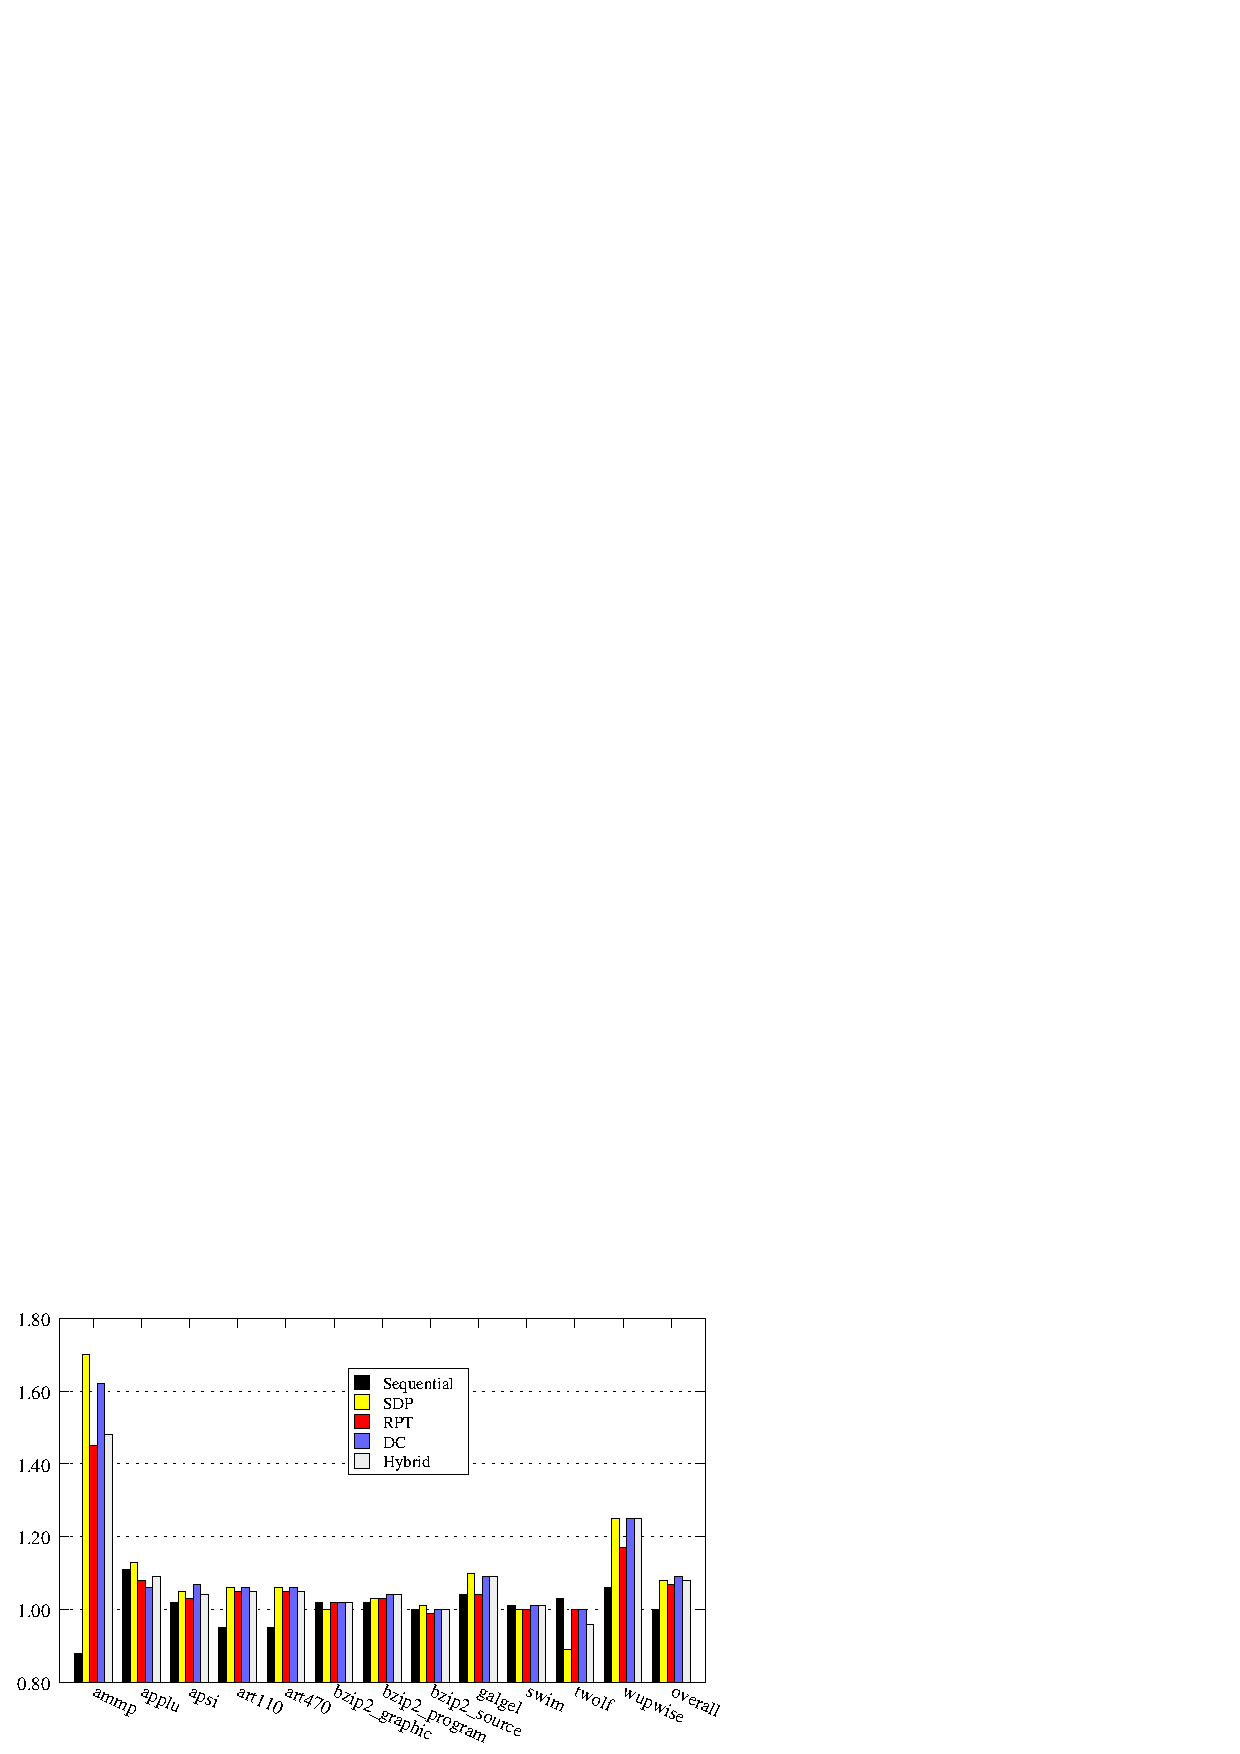
\includegraphics{plots/overview_speedup.pdf}
  \caption{Speedup for each prefetcher for all benchmarks and harmonic mean average speedup.}
  \label{fig:comparison}
\end{figure*}

\begin{figure*}
  \centering
  \includegraphics{plots/accuracy_overview.pdf}
  \caption{Comparison of prefetcher accuracy for all benchmarks.}
  \label{fig:accuracy}
\end{figure*}

\begin{figure*}
  \centering
  \includegraphics{plots/coverage_overview.pdf}
  \caption{Comparison of prefetcher coverage for all benchmarks.}
  \label{fig:coverage}
\end{figure*}


An interesting example of how the different prefetchers differ, is the
\texttt{ammp} benchmark.  \todo{Add figure with the prefetchers' performance on
ammp} This is the benchmark where the sequential prefetcher performs worst; it
degrades performance significantly and a higher prefetching degree only makes
it worse.  For degree 1, it has an extremely low accuracy of only $0.1\%$ which
means most of the effort put into prefetching blocks is wasted.

The SDP prefetcher on the other hand performs quite well and gives a speedup of
$1.7$ for a prefetching degree of $3$. For this degree, an accuracy of $86\%$
means much fewer of the prefetches are wasted effort.  As the only difference
between this and the sequential prefetcher is the variable stride used for SDP,
this indicates that the \texttt{ammp} benchmark accesses memory in a linear,
but strided fashion.  \todo{Is this consistent with the benchmark description?}

The remaining prefetchers all handle strided access and results comparable with
SDP should therefore be expected.  For delta correlation, the best results are
achieved with a prefetching degree of $6$.  At this degree, $84\%$ of the
prefetches turns out to be useful.  The fetches for useless data is probably
what makes delta correlation less effective than SDP despite the improved
coverage.
%TODO: Comment how many of these were already in MSHRs?
This is also suggested by the $44\%$ increase in average cache miss latency.

For the hybrid prefetcher developed during this project, the speedup on \texttt{ammp} is slightly
worse than for the pure delta correlation approach.
Despite falling back to RPT and eventually SDP, the hybrid approach identifies
fewer prefetches than the delta correlating prefetcher.
Combined with about the same accuracy as for delta correlation, this can explain
the reduced performance.
\todo{Why? It should have more}

Another interesting benchmark is \texttt{wupwise}.
\todo{Add figure}
In this benchmark, SDP, delta correlating and hybrid prefetchers all give a
consistent speedup of $1.25$ for all the degrees tested.
RPT is also giving a very consistent speedup of around $1.21$, which is sightly
worse than sequential for degrees greater than 1.
This can be explained if the benchmarks contains long runs of strided memory
access.
Thus the first block after the requested one may not be needed, as assumed in
sequential prefetching, but the next one may be.
As a result, sequential prefetching with a higher degree performs better up to a
certain limit at the maximum stride observed.

Comparing SDP and RPT, both stride based, it becomes clear that the lower
performance of RPT can be explained by a combination of a slightly lower
accuracy and a lower number of identified prefetches.
This may be due to RPT, being more restrictive, only identifies prefetches when
the two last deltas are equal, in contrast to SDP which only requires one.
On the other hand, delta correlation still maintains the same performance while
requiring even more history.
A possible explanation may be that the benchmark's memory access pattern
includes a lot of repeating patterns exploitable by delta correlation.
If the patterns also include some runs of equal deltas, this should be
beneficial to SDP as well because it utilizes shorter runs of equal deltas
better than RPT.

This may also be the reason for the good performance of sequential prefetching
compared to RPT.
From the statistics, RPT only identifies about $72\%$ the number of prefetches
sequential does.
Despite the lower accuracy, this results in a coverage about $15\%$ higher for
sequential.

A noteworthy observation is that the hybrid prefetcher performs comparably to
SDP and delta correlation, even though it follows the RPT policy when there are
only two history entries.
This is natural since delta correlation is always used when possible, otherwise
SDP provides adequate prediction and the few predictions made using RPT does not
affect the overall performance.

The only benchmark where the hybrid prefetcher performs notably worse than the
delta correlating prefetcher is the \texttt{twolf} benchmark.
Comparing the number of identified prefetches, the hybrid prefetcher identifies
about $10$ times as many as the delta correlating prefetcher.
These prefetches do not turn out to be beneficial in most cases as can be seen
from the lower accuracy of the hybrid prefetcher.

Since the hybrid approach uses the same strategy as SDP and RPT when too little
history is available for delta correlation, poor performance for RPT and SDP is
also to be expected.
This proves to be the case as well; the SDP prefetcher has the absolutely worst
performance.
Even though it identifies almost the same number of prefetches as the much
better performing RPT, it falls short on accuracy.

An example where the hybrid prefetcher actually performs better than the delta
correlating prefetcher can be found by looking at the \texttt{applu} benchmark.
This happens for degrees ranging from $1$ to $4$, which is due to a higher
number of identified prefetches by the hybrid implementation while both
prefetches maintain an accuracy above $90\%$.

Furthermore, we have an example of the sequential prefetcher performing much
better than all the stride based prefetchers for all degrees above 1.
This may be due to very irregular strides, causing the stride based prefetchers
to fetch useless blocks, which degrades performance.


// TODO: Write more in depth analysis that explore why the hybrid prefetcher performs worse than DC.


%The best average speedup is $1.0$ for a degree of 1.
%We observe that different benchmarks respond differently to different degrees of prefetching.
%See Figure \ref{fig:sequential}
%\texttt{applu},
%
%
%\begin{figure}
%  \input{plots/sequential.tex}
%  \caption{Effect of prefetching degree in sequential prefetcher for benchmarks.}
%  \label{fig:sequential}
%\end{figure}
%
%%\begin{figure*}
%%  \input{plots/seq3.tex}
%%  \caption{Performance of sequential prefetcher with $p = 3$ across benchmarks.}
%%  \label{fig:seq3}
%%\end{figure*}
%
%\subsubsection{Stride Direct Prefetcher}
%A simple implementation of a stride direct prefetcher yielded a better average speedup ($1.07$) than the sequential prefetcher.
%The benchmarks wupwise and ammp had high speedups, which pulled up the average.
%This prefetcher had a negative impact on the twolf benchmark.
%
%
%\subsubsection{Reference Prediction Table}
%// TODO: 
%The RPT implementation yielded an average speedup of $1.06$.
%While slightly lower than the SDP average, the maximum and minimum values are closer together.
%Testing of the RPT implementation saw no benchmark with a speedup of less than $0.95$.
%Figure~\ref{fig:rpt} shows how RPT performs on each benchmark.
%
%%\begin{figure*}
%%  % GNUPLOT: LaTeX picture with Postscript
\begingroup
  \makeatletter
  \providecommand\color[2][]{%
    \GenericError{(gnuplot) \space\space\space\@spaces}{%
      Package color not loaded in conjunction with
      terminal option `colourtext'%
    }{See the gnuplot documentation for explanation.%
    }{Either use 'blacktext' in gnuplot or load the package
      color.sty in LaTeX.}%
    \renewcommand\color[2][]{}%
  }%
  \providecommand\includegraphics[2][]{%
    \GenericError{(gnuplot) \space\space\space\@spaces}{%
      Package graphicx or graphics not loaded%
    }{See the gnuplot documentation for explanation.%
    }{The gnuplot epslatex terminal needs graphicx.sty or graphics.sty.}%
    \renewcommand\includegraphics[2][]{}%
  }%
  \providecommand\rotatebox[2]{#2}%
  \@ifundefined{ifGPcolor}{%
    \newif\ifGPcolor
    \GPcolorfalse
  }{}%
  \@ifundefined{ifGPblacktext}{%
    \newif\ifGPblacktext
    \GPblacktexttrue
  }{}%
  % define a \g@addto@macro without @ in the name:
  \let\gplgaddtomacro\g@addto@macro
  % define empty templates for all commands taking text:
  \gdef\gplbacktext{}%
  \gdef\gplfronttext{}%
  \makeatother
  \ifGPblacktext
    % no textcolor at all
    \def\colorrgb#1{}%
    \def\colorgray#1{}%
  \else
    % gray or color?
    \ifGPcolor
      \def\colorrgb#1{\color[rgb]{#1}}%
      \def\colorgray#1{\color[gray]{#1}}%
      \expandafter\def\csname LTw\endcsname{\color{white}}%
      \expandafter\def\csname LTb\endcsname{\color{black}}%
      \expandafter\def\csname LTa\endcsname{\color{black}}%
      \expandafter\def\csname LT0\endcsname{\color[rgb]{1,0,0}}%
      \expandafter\def\csname LT1\endcsname{\color[rgb]{0,1,0}}%
      \expandafter\def\csname LT2\endcsname{\color[rgb]{0,0,1}}%
      \expandafter\def\csname LT3\endcsname{\color[rgb]{1,0,1}}%
      \expandafter\def\csname LT4\endcsname{\color[rgb]{0,1,1}}%
      \expandafter\def\csname LT5\endcsname{\color[rgb]{1,1,0}}%
      \expandafter\def\csname LT6\endcsname{\color[rgb]{0,0,0}}%
      \expandafter\def\csname LT7\endcsname{\color[rgb]{1,0.3,0}}%
      \expandafter\def\csname LT8\endcsname{\color[rgb]{0.5,0.5,0.5}}%
    \else
      % gray
      \def\colorrgb#1{\color{black}}%
      \def\colorgray#1{\color[gray]{#1}}%
      \expandafter\def\csname LTw\endcsname{\color{white}}%
      \expandafter\def\csname LTb\endcsname{\color{black}}%
      \expandafter\def\csname LTa\endcsname{\color{black}}%
      \expandafter\def\csname LT0\endcsname{\color{black}}%
      \expandafter\def\csname LT1\endcsname{\color{black}}%
      \expandafter\def\csname LT2\endcsname{\color{black}}%
      \expandafter\def\csname LT3\endcsname{\color{black}}%
      \expandafter\def\csname LT4\endcsname{\color{black}}%
      \expandafter\def\csname LT5\endcsname{\color{black}}%
      \expandafter\def\csname LT6\endcsname{\color{black}}%
      \expandafter\def\csname LT7\endcsname{\color{black}}%
      \expandafter\def\csname LT8\endcsname{\color{black}}%
    \fi
  \fi
    \setlength{\unitlength}{0.0500bp}%
    \ifx\gptboxheight\undefined%
      \newlength{\gptboxheight}%
      \newlength{\gptboxwidth}%
      \newsavebox{\gptboxtext}%
    \fi%
    \setlength{\fboxrule}{0.5pt}%
    \setlength{\fboxsep}{1pt}%
\begin{picture}(7200.00,5040.00)%
    \gplgaddtomacro\gplbacktext{%
      \csname LTb\endcsname%
      \put(814,2263){\makebox(0,0)[r]{\strut{}$0.5$}}%
      \put(814,2545){\makebox(0,0)[r]{\strut{}$0.6$}}%
      \put(814,2827){\makebox(0,0)[r]{\strut{}$0.7$}}%
      \put(814,3109){\makebox(0,0)[r]{\strut{}$0.8$}}%
      \put(814,3392){\makebox(0,0)[r]{\strut{}$0.9$}}%
      \put(814,3674){\makebox(0,0)[r]{\strut{}$1$}}%
      \put(814,3956){\makebox(0,0)[r]{\strut{}$1.1$}}%
      \put(814,4238){\makebox(0,0)[r]{\strut{}$1.2$}}%
      \put(1190,2068){\rotatebox{-270}{\makebox(0,0)[r]{\strut{}bzip2-source}}}%
      \put(1678,2068){\rotatebox{-270}{\makebox(0,0)[r]{\strut{}twolf}}}%
      \put(2166,2068){\rotatebox{-270}{\makebox(0,0)[r]{\strut{}swim}}}%
      \put(2654,2068){\rotatebox{-270}{\makebox(0,0)[r]{\strut{}apsi}}}%
      \put(3142,2068){\rotatebox{-270}{\makebox(0,0)[r]{\strut{}galgel}}}%
      \put(3630,2068){\rotatebox{-270}{\makebox(0,0)[r]{\strut{}bzip2-graphic}}}%
      \put(4119,2068){\rotatebox{-270}{\makebox(0,0)[r]{\strut{}art110}}}%
      \put(4607,2068){\rotatebox{-270}{\makebox(0,0)[r]{\strut{}art470}}}%
      \put(5095,2068){\rotatebox{-270}{\makebox(0,0)[r]{\strut{}bzip2-program}}}%
      \put(5583,2068){\rotatebox{-270}{\makebox(0,0)[r]{\strut{}applu}}}%
      \put(6071,2068){\rotatebox{-270}{\makebox(0,0)[r]{\strut{}wupwise}}}%
      \put(6559,2068){\rotatebox{-270}{\makebox(0,0)[r]{\strut{}ammp}}}%
    }%
    \gplgaddtomacro\gplfronttext{%
      \csname LTb\endcsname%
      \put(176,3321){\rotatebox{-270}{\makebox(0,0){\strut{}Speedup}}}%
      \put(3874,154){\makebox(0,0){\strut{}Benchmark}}%
      \put(3874,4709){\makebox(0,0){\strut{}Reference Prediction Table}}%
    }%
    \gplbacktext
    \put(0,0){\includegraphics{plots/rpt}}%
    \gplfronttext
  \end{picture}%
\endgroup

%%  \caption{Performance of RPT prefetcher across benchmarks.}
%%  \label{fig:rpt}
%%\end{figure*}
%
%\subsubsection{Global History Buffer with Delta Correlation}
%The implementation of the global history buffer with SDP and RTP as fallback was successfully implemented and yielded the speedups shown in Figure \ref{fig:ghbdc}.
%The best speedup was acquired for the ammp benchmark, but many of the other benchmark showed only a slight speedup if any at all.
%
%
%\begin{figure*}
%  % GNUPLOT: LaTeX picture with Postscript
\begingroup
  \makeatletter
  \providecommand\color[2][]{%
    \GenericError{(gnuplot) \space\space\space\@spaces}{%
      Package color not loaded in conjunction with
      terminal option `colourtext'%
    }{See the gnuplot documentation for explanation.%
    }{Either use 'blacktext' in gnuplot or load the package
      color.sty in LaTeX.}%
    \renewcommand\color[2][]{}%
  }%
  \providecommand\includegraphics[2][]{%
    \GenericError{(gnuplot) \space\space\space\@spaces}{%
      Package graphicx or graphics not loaded%
    }{See the gnuplot documentation for explanation.%
    }{The gnuplot epslatex terminal needs graphicx.sty or graphics.sty.}%
    \renewcommand\includegraphics[2][]{}%
  }%
  \providecommand\rotatebox[2]{#2}%
  \@ifundefined{ifGPcolor}{%
    \newif\ifGPcolor
    \GPcolorfalse
  }{}%
  \@ifundefined{ifGPblacktext}{%
    \newif\ifGPblacktext
    \GPblacktexttrue
  }{}%
  % define a \g@addto@macro without @ in the name:
  \let\gplgaddtomacro\g@addto@macro
  % define empty templates for all commands taking text:
  \gdef\gplbacktext{}%
  \gdef\gplfronttext{}%
  \makeatother
  \ifGPblacktext
    % no textcolor at all
    \def\colorrgb#1{}%
    \def\colorgray#1{}%
  \else
    % gray or color?
    \ifGPcolor
      \def\colorrgb#1{\color[rgb]{#1}}%
      \def\colorgray#1{\color[gray]{#1}}%
      \expandafter\def\csname LTw\endcsname{\color{white}}%
      \expandafter\def\csname LTb\endcsname{\color{black}}%
      \expandafter\def\csname LTa\endcsname{\color{black}}%
      \expandafter\def\csname LT0\endcsname{\color[rgb]{1,0,0}}%
      \expandafter\def\csname LT1\endcsname{\color[rgb]{0,1,0}}%
      \expandafter\def\csname LT2\endcsname{\color[rgb]{0,0,1}}%
      \expandafter\def\csname LT3\endcsname{\color[rgb]{1,0,1}}%
      \expandafter\def\csname LT4\endcsname{\color[rgb]{0,1,1}}%
      \expandafter\def\csname LT5\endcsname{\color[rgb]{1,1,0}}%
      \expandafter\def\csname LT6\endcsname{\color[rgb]{0,0,0}}%
      \expandafter\def\csname LT7\endcsname{\color[rgb]{1,0.3,0}}%
      \expandafter\def\csname LT8\endcsname{\color[rgb]{0.5,0.5,0.5}}%
    \else
      % gray
      \def\colorrgb#1{\color{black}}%
      \def\colorgray#1{\color[gray]{#1}}%
      \expandafter\def\csname LTw\endcsname{\color{white}}%
      \expandafter\def\csname LTb\endcsname{\color{black}}%
      \expandafter\def\csname LTa\endcsname{\color{black}}%
      \expandafter\def\csname LT0\endcsname{\color{black}}%
      \expandafter\def\csname LT1\endcsname{\color{black}}%
      \expandafter\def\csname LT2\endcsname{\color{black}}%
      \expandafter\def\csname LT3\endcsname{\color{black}}%
      \expandafter\def\csname LT4\endcsname{\color{black}}%
      \expandafter\def\csname LT5\endcsname{\color{black}}%
      \expandafter\def\csname LT6\endcsname{\color{black}}%
      \expandafter\def\csname LT7\endcsname{\color{black}}%
      \expandafter\def\csname LT8\endcsname{\color{black}}%
    \fi
  \fi
  \setlength{\unitlength}{0.0500bp}%
  \begin{picture}(10204.00,2834.00)%
    \gplgaddtomacro\gplbacktext{%
      \csname LTb\endcsname%
      \put(946,704){\makebox(0,0)[r]{\strut{} 1}}%
      \put(946,970){\makebox(0,0)[r]{\strut{} 1.1}}%
      \put(946,1237){\makebox(0,0)[r]{\strut{} 1.2}}%
      \put(946,1503){\makebox(0,0)[r]{\strut{} 1.3}}%
      \put(946,1770){\makebox(0,0)[r]{\strut{} 1.4}}%
      \put(946,2036){\makebox(0,0)[r]{\strut{} 1.5}}%
      \put(946,2303){\makebox(0,0)[r]{\strut{} 1.6}}%
      \put(946,2569){\makebox(0,0)[r]{\strut{} 1.7}}%
      \put(1518,484){\makebox(0,0){\strut{} 1}}%
      \put(2398,484){\makebox(0,0){\strut{} 2}}%
      \put(3277,484){\makebox(0,0){\strut{} 3}}%
      \put(4157,484){\makebox(0,0){\strut{} 4}}%
      \put(5037,484){\makebox(0,0){\strut{} 5}}%
      \put(5916,484){\makebox(0,0){\strut{} 6}}%
      \put(6796,484){\makebox(0,0){\strut{} 7}}%
      \put(176,1636){\rotatebox{-270}{\makebox(0,0){\strut{}Speedup}}}%
      \put(4157,154){\makebox(0,0){\strut{}Prefetching degree}}%
    }%
    \gplgaddtomacro\gplfronttext{%
      \csname LTb\endcsname%
      \put(9216,2459){\makebox(0,0)[r]{\strut{}ammp}}%
      \csname LTb\endcsname%
      \put(9216,2239){\makebox(0,0)[r]{\strut{}applu}}%
      \csname LTb\endcsname%
      \put(9216,2019){\makebox(0,0)[r]{\strut{}apsi}}%
      \csname LTb\endcsname%
      \put(9216,1799){\makebox(0,0)[r]{\strut{}art110}}%
      \csname LTb\endcsname%
      \put(9216,1579){\makebox(0,0)[r]{\strut{}art470}}%
      \csname LTb\endcsname%
      \put(9216,1359){\makebox(0,0)[r]{\strut{}bzip2-graphic}}%
      \csname LTb\endcsname%
      \put(9216,1139){\makebox(0,0)[r]{\strut{}bzip2-program}}%
    }%
    \gplbacktext
    \put(0,0){\includegraphics{ghbdc}}%
    \gplfronttext
  \end{picture}%
\endgroup

%  \caption{Speedup of each benchmark as a function of degree for the global history buffer with delta correlation and fall back to SDP and RTP.}
%  \label{fig:ghbdc}
%\end{figure*}
%
%\begin{figure*}
%  \input{plots/ghbdcavg.tex}
%  \caption{Average speedup as a function of prefetching degree for our final prefetcher implementation.}
%  \label{fig:ghbdcavg}
%\end{figure*}
%
%%\subsection{Description}
%% This section might elaborate on alternative approaches that
%% you have tried, but were not successful. It discusses weaknesses
%% of your scheme and highlights the strong and weak
%% points of your experimental setup.
%
%Experimenting with sequential prefetching of various degrees yielded surprisingly good results for some benchmarks.
%A possible explanation for this is that the benchmark's behavior matched exceptionally well with the assumptions used when creating the prefetcher.
%Based on this, it is reasonable to assume that the \texttt{applu} and \texttt{wupwise} benchmarks access memory fairly sequentially.
%
%\todo{SDP}
%\todo{RPT}
%
%Our hybrid implementation
%More interesting to note, is that the delta-correlation implementation does an exceptionally good job at the \texttt{ammp} benchmark.
%This was the benchmark with the highest negative performance impact from the naive sequential prefetcher, but the memory pattern seems to be very well suited for delta correlation.
